\documentclass[aspectratio=169]{beamer}
%[handout]

\usetheme[progressbar=frametitle]{metropolis}
\usepackage{appendixnumberbeamer}

\usepackage[utf8]{inputenc}
\usepackage[T1]{fontenc}

\usepackage[brazil]{babel}
\usepackage[outputdir=..]{minted}
\usepackage{xcolor}
\usepackage{soul} % strikethrough
\usepackage{advdate}
\usepackage{graphicx}
\graphicspath{{figs/}}
\usepackage{graphbox}

\usepackage[ampersand]{easylist}

\usepackage{multirow}
\usepackage{multicol}
\usepackage{subcaption}

\usepackage{pgf,tikz}
\usetikzlibrary{shapes,arrows,positioning}
\usetikzlibrary{circuits.logic.US}
\usetikzlibrary{matrix,calc}

\usepackage{karnaugh-map}

\usepackage{pgfpages}
\setbeameroption{hide notes} % Only slides
% \setbeameroption{show only notes} % Only notes
% \setbeameroption{show notes on second screen=right} % Both

% \graphicspath{{../figs/}}

\definecolor{bgc}{rgb}{0.95,0.9,0.95}
\definecolor{links}{HTML}{2A7F7F}
\hypersetup{colorlinks,linkcolor=,urlcolor=links}

\newminted{verilog}{fontsize=\scriptsize, 
    linenos,
    numbersep=8pt,
    bgcolor=bgc,
    tabsize=4,
    framesep=3mm} 
    %frame=lines,

\newcommand{\verilog}[1]{\verilogf{#1}{\footnotesize}}

\newcommand{\verilogf}[2]{\inputminted[fontsize=#2, 
    linenos,
    tabsize=2,
    numbersep=4pt,
    bgcolor=bgc,
    framesep=3mm]{verilog}{../codes/#1.v}
}

\newminted{nasm}{fontsize=\scriptsize, 
		   linenos,
		   numbersep=8pt,
           bgcolor=bgc,
		   framesep=3mm} 

\usepackage{booktabs}
\usepackage[scale=2]{ccicons}

\usepackage{pgfplots}
\usepgfplotslibrary{dateplot}

\usepackage{hyperref}


\usepackage{xspace}
\newcommand{\themename}{\textbf{\textsc{metropolis}}\xspace}



\usepackage{pifont}% http://ctan.org/pkg/pifont
\newcommand{\cmark}{\ding{51}}%
\newcommand{\xmark}{\ding{55}}%

% \tiny	
% \scriptsize
% \footnotesize
% \small	
% \normalsize	
% \large	
% \Large	
% \LARGE	
% \huge	
% \Huge	



\newminted{python}{fontsize=\scriptsize, 
		   linenos,
		   breaklines,
		   numbersep=8pt,
           tabsize=2,
		   framesep=3mm} 
		   
\newminted{verilog}{fontsize=\scriptsize, 
		   linenos,
		   breaklines,
		   numbersep=8pt,
           tabsize=2,
		   framesep=3mm} 
		   




\definecolor{bgc}{rgb}{0.95,0.9,0.95}
\definecolor{links}{HTML}{2A7F7F}
\hypersetup{colorlinks,linkcolor=,urlcolor=links}


% \usepackage[style=apa]{biblatex}
% \addbibresource{mm.bib}


% \author{\large Prof. Ricardo Menotti (\href{mailto:menotti@ufscar.br}{menotti@ufscar.br})}

\newcommand{\newauthor}[2]{
  \parbox{0.50\textwidth}{
    \texorpdfstring
      {
        \centering
        \small #1 \newline
        {\scriptsize{\urlstyle{same}\href{mailto:#2}{#2}\urlstyle{tt}}}
      }
      {#1} \newline
  }
}

\author{
  \newauthor{Prof. Ricardo Menotti}{menotti@ufscar.br}
\and \newauthor{Prof. Luciano de Oliveira Neris}{lneris@ufscar.br}  
%\and \newauthor{Prof. Artino Quintino da Silva Filho}{artino@ufscar.br}
% \and \newauthor{Prof. Maurício Figueiredo}{mauricio@ufscar.br}
% \and \newauthor{Prof. Edilson Kato}{kato@ufscar.br}
% \and \newauthor{Prof. Roberto Inoue}{rsinoue@ufscar.br}
}

\date{Atualizado em: \today}

\institute{\large \textbf{Departamento de Computação} \\
Centro de Ciências Exatas e de Tecnologia \\
Universidade Federal de São Carlos}

\title{Lógica Digital (1001351)}

\titlegraphic{\hfill
\includegraphics[height=1.5cm]{LogoUfscar}}



\subtitle{Mapas de Karnaugh} % 

% https://tex.stackexchange.com/questions/140567/drawing-karnaughs-maps-in-latex
% http://www.texample.net/tikz/examples/karnaugh-diagram/

\begin{document}

\begin{frame}
	\titlepage
\end{frame} 

%%%%%%%%%%%%%%%%%%%%%%%%%%%%%%%%%%%%%%%%%%%%%%%%%%%%%%%%%%%%%%%%%%%%%%%%%%%%%%%%

\section{Mapas de Karnaugh}

\begin{frame}{\insertsection: produto das somas}
    \begin{columns}
        \begin{column}{0.50\textwidth}
            \vspace{3cm}
            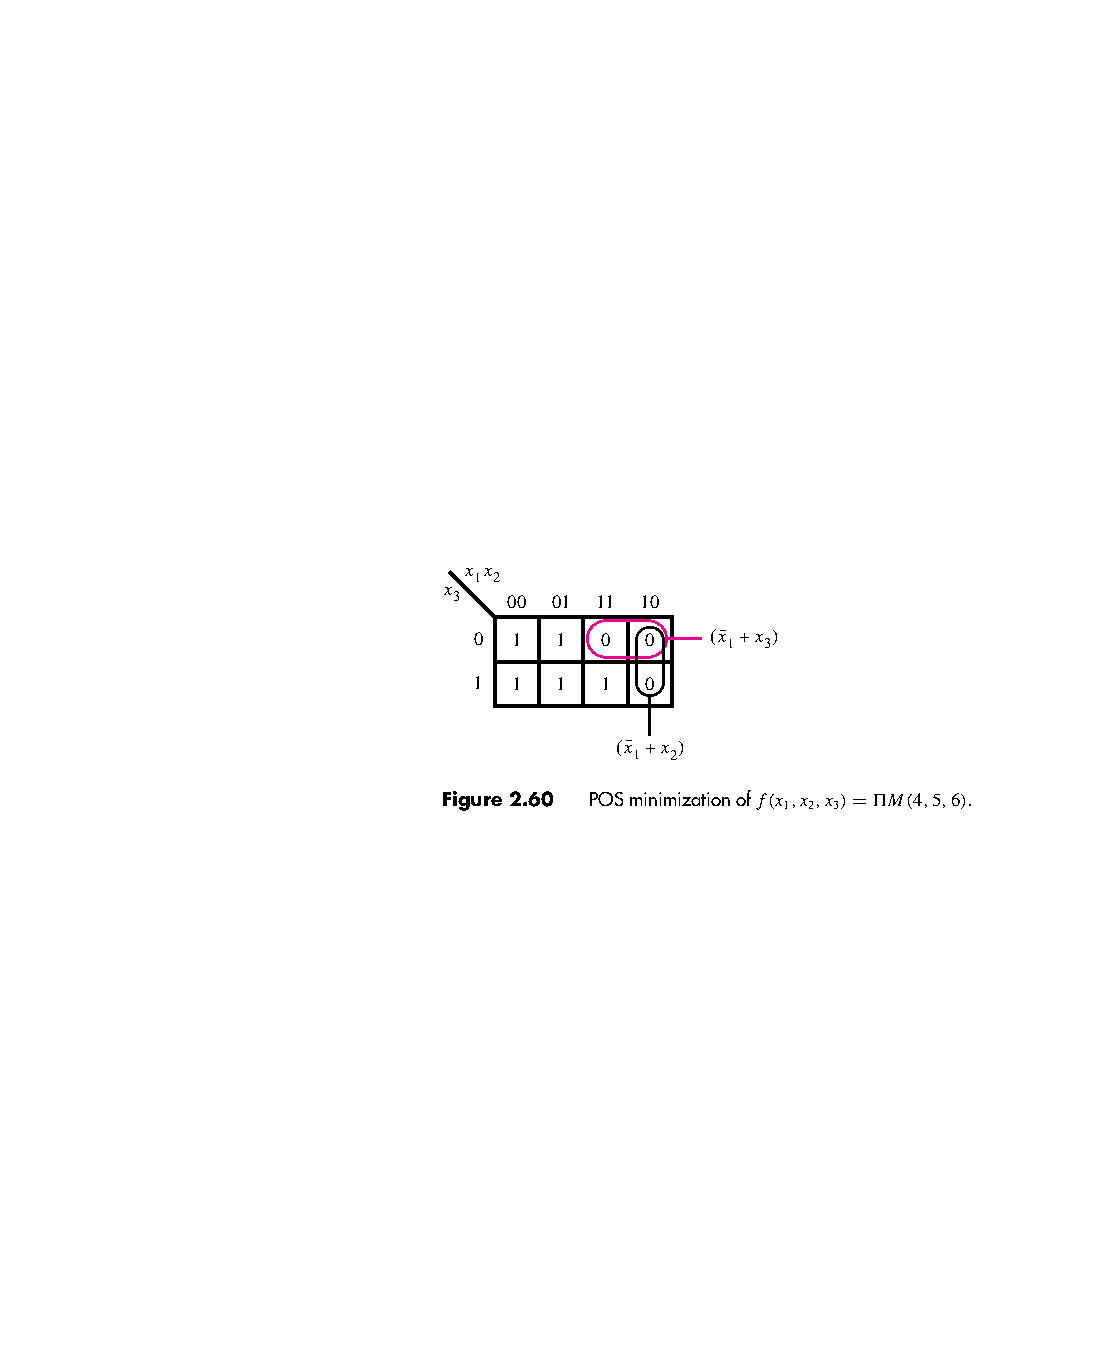
\includegraphics[width=1.5\textwidth]{VerilogFig2_60}
        \end{column}        
        \begin{column}{0.50\textwidth}
            \small
            \begin{tabular}{rl}
            $f=$ & $(\overline{x}_1 + x_2)(\overline{x}_1+x_3)$ \\[2ex]
            \pause
            $\overline{f}=$ & $x_1\overline{x}_2 + x_1\overline{x}_3$ \\[2ex]
            $f=\overline{\overline{f}}=$ & $\overline{x_1\overline{x}_2 + x_1\overline{x}_3}$ \\[2ex]
            $f=$ & $\overline{x_1\overline{x}_2}.\overline{x_1\overline{x}_3}$ \\[2ex]
            $f=$ & $(\overline{x}_1 + x_2)(\overline{x}_1+x_3)$ \\[2ex]
            \pause
            $f=$ & $\overline{x}_1 + x_2x_3$ \\[2ex]
            \end{tabular}
        \end{column}
    \end{columns}
\end{frame}

\begin{frame}{\insertsection: produto das somas}
    \centering
    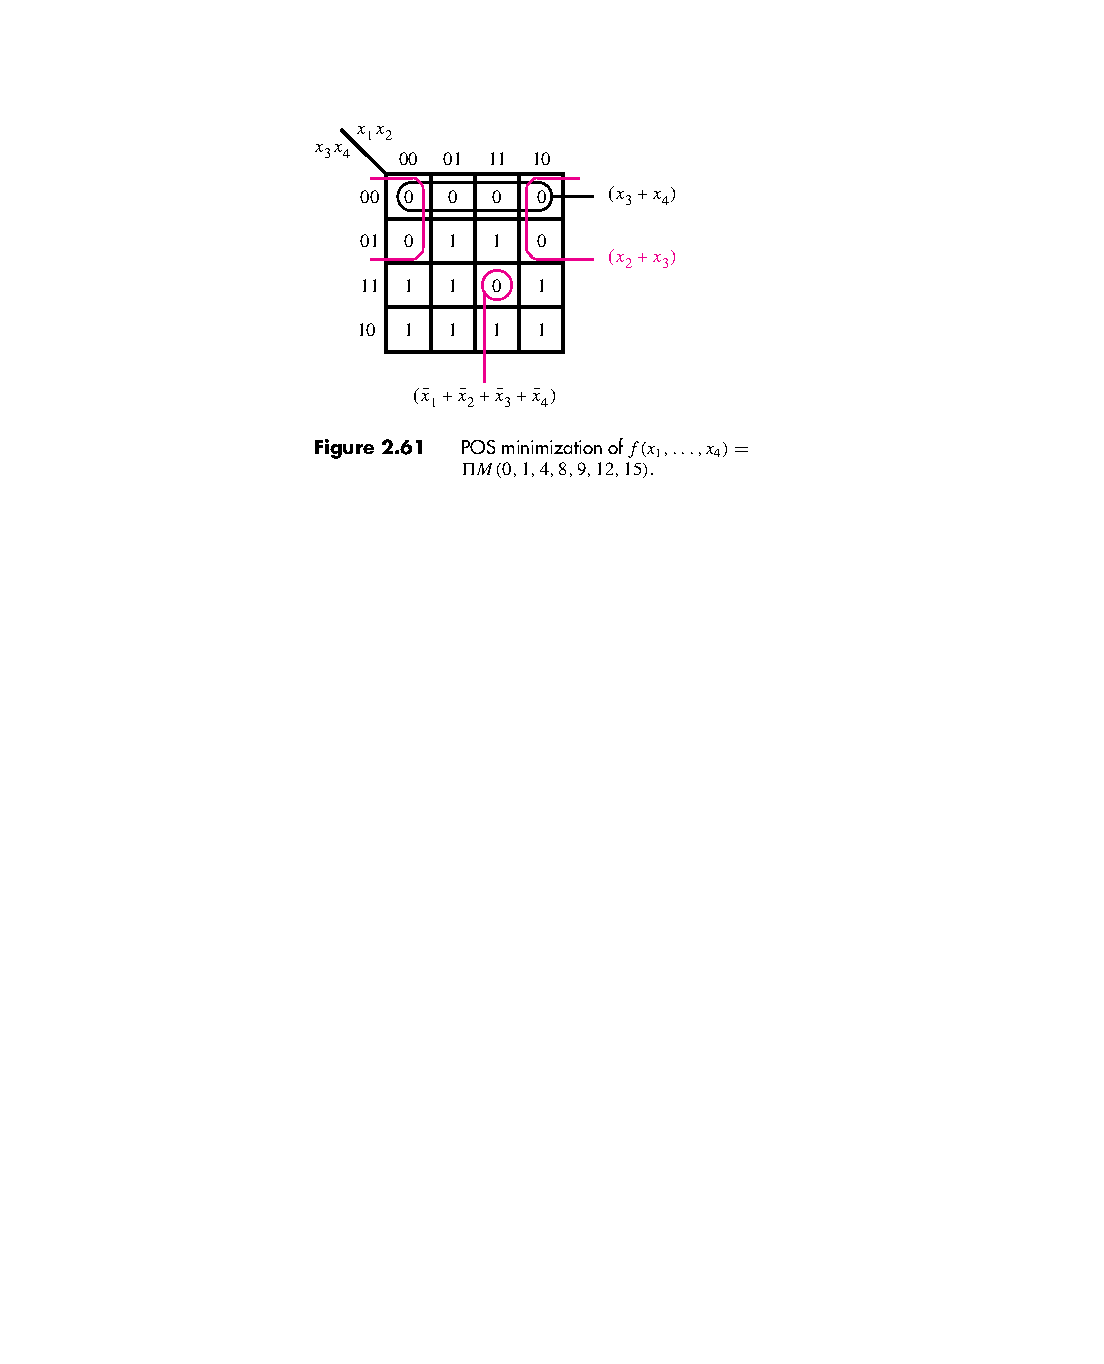
\includegraphics[width=.65\textwidth]{VerilogFig2_61}
\end{frame}

\section{Especificação incompleta \\(don't care)}

\begin{frame}{\insertsection}
    \begin{itemize}
        \item Nos circuitos digitais, há certas situações onde algumas entradas para uma função nunca acontecem. Ex:
        \begin{itemize}
            \item Um sensor para detectar se uma porta está aberta e outro para detectar se a mesma porta está fechada;
            \item Um sensor para detectar se um objeto é muito pesado e outro se ele é muito leve; etc. 
        \end{itemize}
        \item Em funções deste tipo, as entradas que nunca ocorrem são chamadas de \textit{\textbf{indiferenças} (don't care conditions)};
        \begin{itemize}
            \item Tanto faz qual será a saída da função nesses casos, já que a entrada nunca ocorre;
            \item Isso pode ser usada para otimizar a função, adotando 0 ou 1 na saída de acordo com a conveniência.
        \end{itemize}
    \end{itemize}
\end{frame}

\begin{frame}{\insertsection}
    \centering
    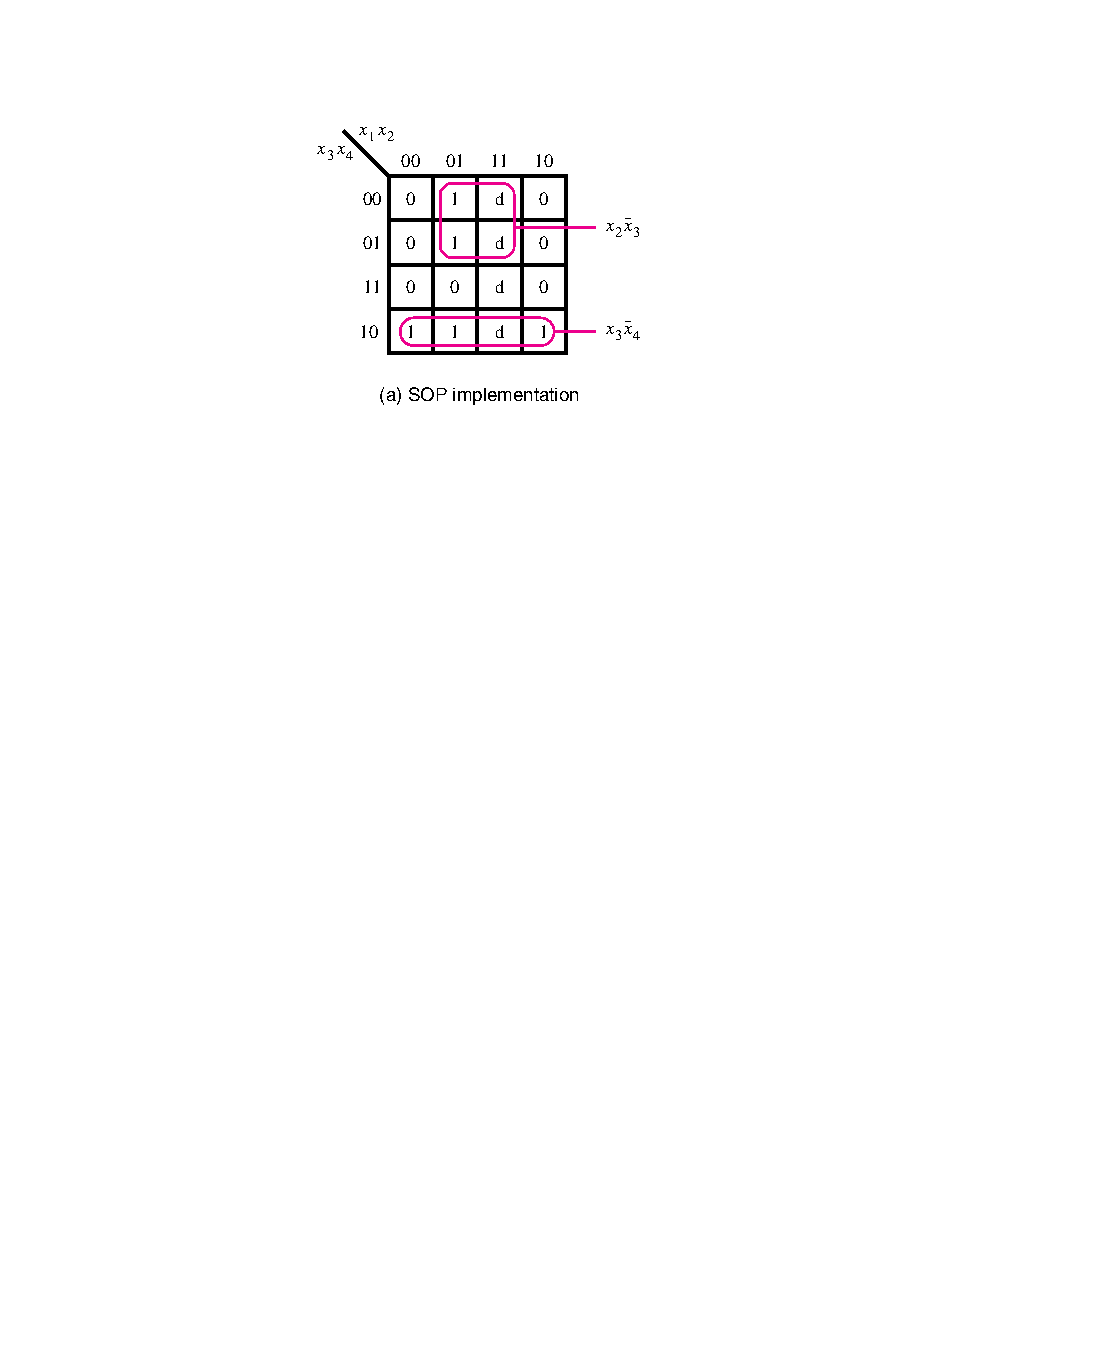
\includegraphics[scale=1]{VerilogFig2_62a}    
    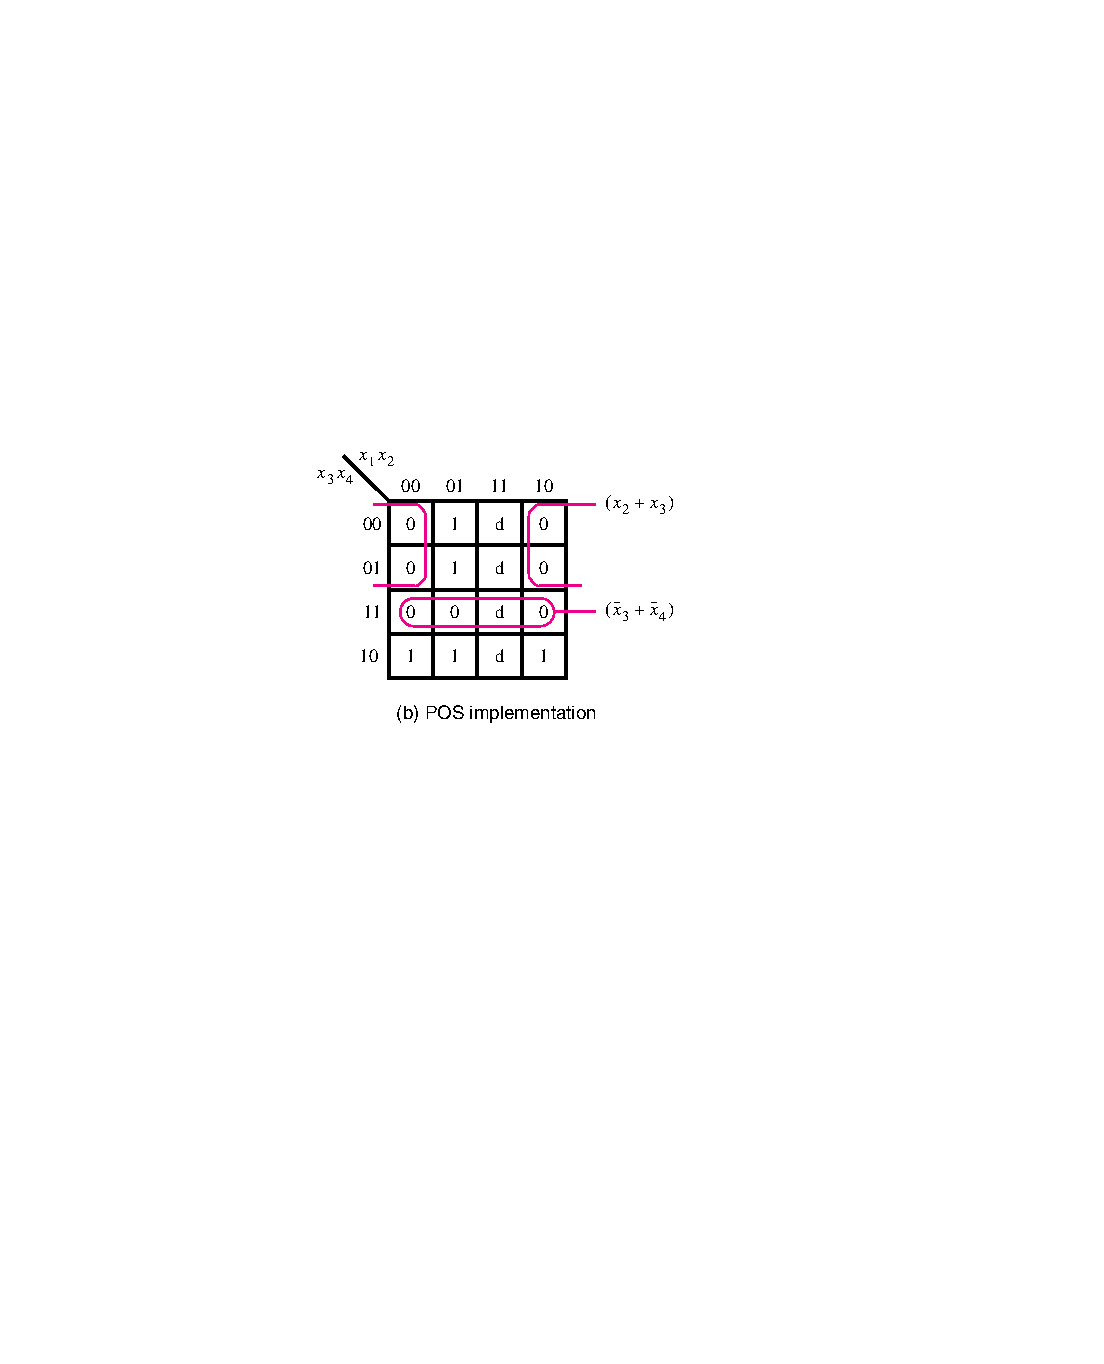
\includegraphics[scale=1]{VerilogFig2_62b}

    $f(x_1,x_2,x_3,x_4)=\Sigma m(2, 4, 5, 6, 10) + D(12, 13, 14, 15)$
\end{frame}

\begin{frame}{\insertsection}
    \begin{columns}
        \begin{column}{0.40\textwidth}
        \scriptsize
        \begin{tabular}{c||c|c|c|c||c} % center, left or right 
            \hline
            BCD & $b_3$ & $b_2$ & $b_1$ & $b_0$ & $f$ \\
            \hline
            \hline
            $0$ & $0$ & $0$ & $0$ & $0$ & $0$ \\
            $1$ & $0$ & $0$ & $0$ & $1$ & $0$ \\
            $2$ & $0$ & $0$ & $1$ & $0$ & $0$ \\
            $3$ & $0$ & $0$ & $1$ & $1$ & $1$ \\
            $4$ & $0$ & $1$ & $0$ & $0$ & $0$ \\
            $5$ & $0$ & $1$ & $0$ & $1$ & $0$ \\
            $6$ & $0$ & $1$ & $1$ & $0$ & $1$ \\
            $7$ & $0$ & $1$ & $1$ & $1$ & $0$ \\
            $8$ & $1$ & $0$ & $0$ & $0$ & $0$ \\
            $9$ & $1$ & $0$ & $0$ & $1$ & $1$ \\
            $A$ & $1$ & $0$ & $1$ & $0$ & $-$ \\
            $b$ & $1$ & $0$ & $1$ & $1$ & $-$ \\
            $C$ & $1$ & $1$ & $0$ & $0$ & $-$ \\
            $d$ & $1$ & $1$ & $0$ & $1$ & $-$ \\
            $E$ & $1$ & $1$ & $1$ & $0$ & $-$ \\
            $F$ & $1$ & $1$ & $1$ & $1$ & $-$ \\
            \hline
        \end{tabular} \\
        \end{column}
        \begin{column}{0.60\textwidth}
    \begin{karnaugh-map}[4][4][1][$x_1x_0$][$x_3x_2$]
    %   \manualterms{0,1,2,3,4,5,6,7,8,9,10,11,12,13,14,15}
      \minterms{3,6,9}
      \terms{10,11,12,13,14,15}{D}
      \autoterms[0]
      \onslide<2>{
      \implicant{3}{3}
      \implicant{6}{6}
      \implicant{9}{9}
      }
      \onslide<3>{
      \implicantedge{3}{3}{11}{11}
      \implicant{6}{14}
      \implicant{13}{11}
      }
    \end{karnaugh-map} \\
    \end{column}        
    \end{columns}
    \centering
        Implementar $f(b_3,b_2,b_1,b_0)=\Sigma m_{(3,6,9)} + D_{(10,11,12,13,14,15)}$
\end{frame}

\section{Circuitos com múltiplas saídas}

\begin{frame}{\insertsection} % Slide with bullets
	\begin{itemize}
		\item Frequentemente é necessário implementar funções que são parte de um sistema maior;
		\item Pode ser possível compartilhar algumas das portas necessárias na implementação de funções individuais;
		\item Essa estratégia nem sempre funciona da melhor maneira, como veremos a seguir;
        \item Em vez de derivar as expressões individualmente, podemos procurar implicantes que possam ser compartilhados com vantagem na realização combinada das funções.
    \end{itemize}
\end{frame}

\begin{frame}{\insertsection} \centering
    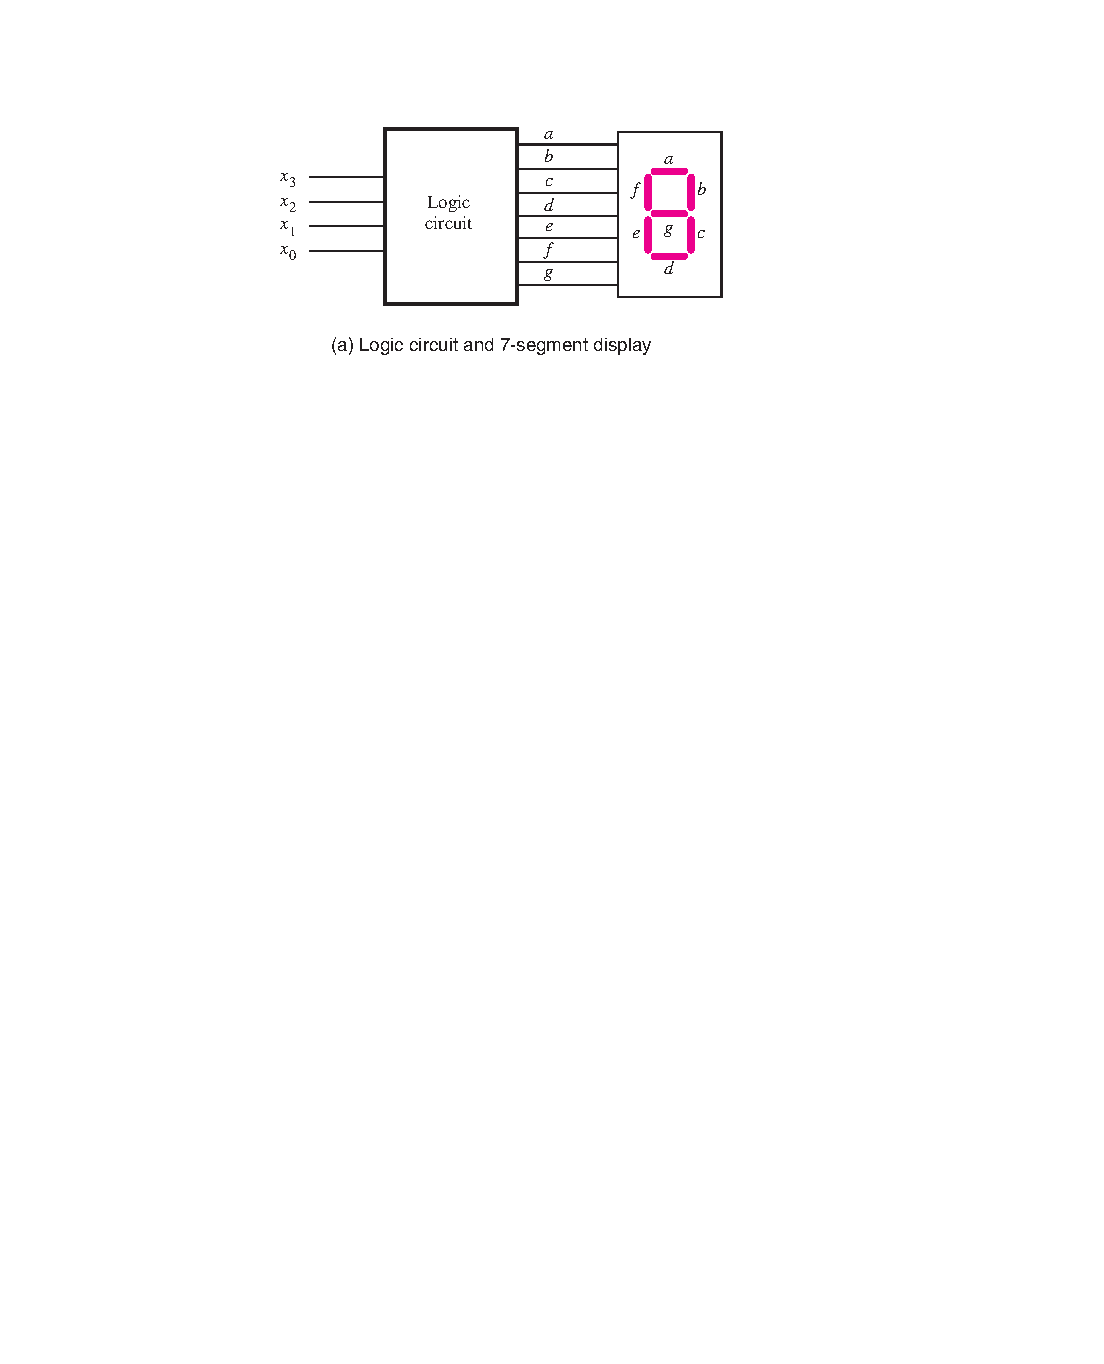
\includegraphics[width=.45\textwidth]{VerilogFig2_63a}
    \hspace{1cm}
    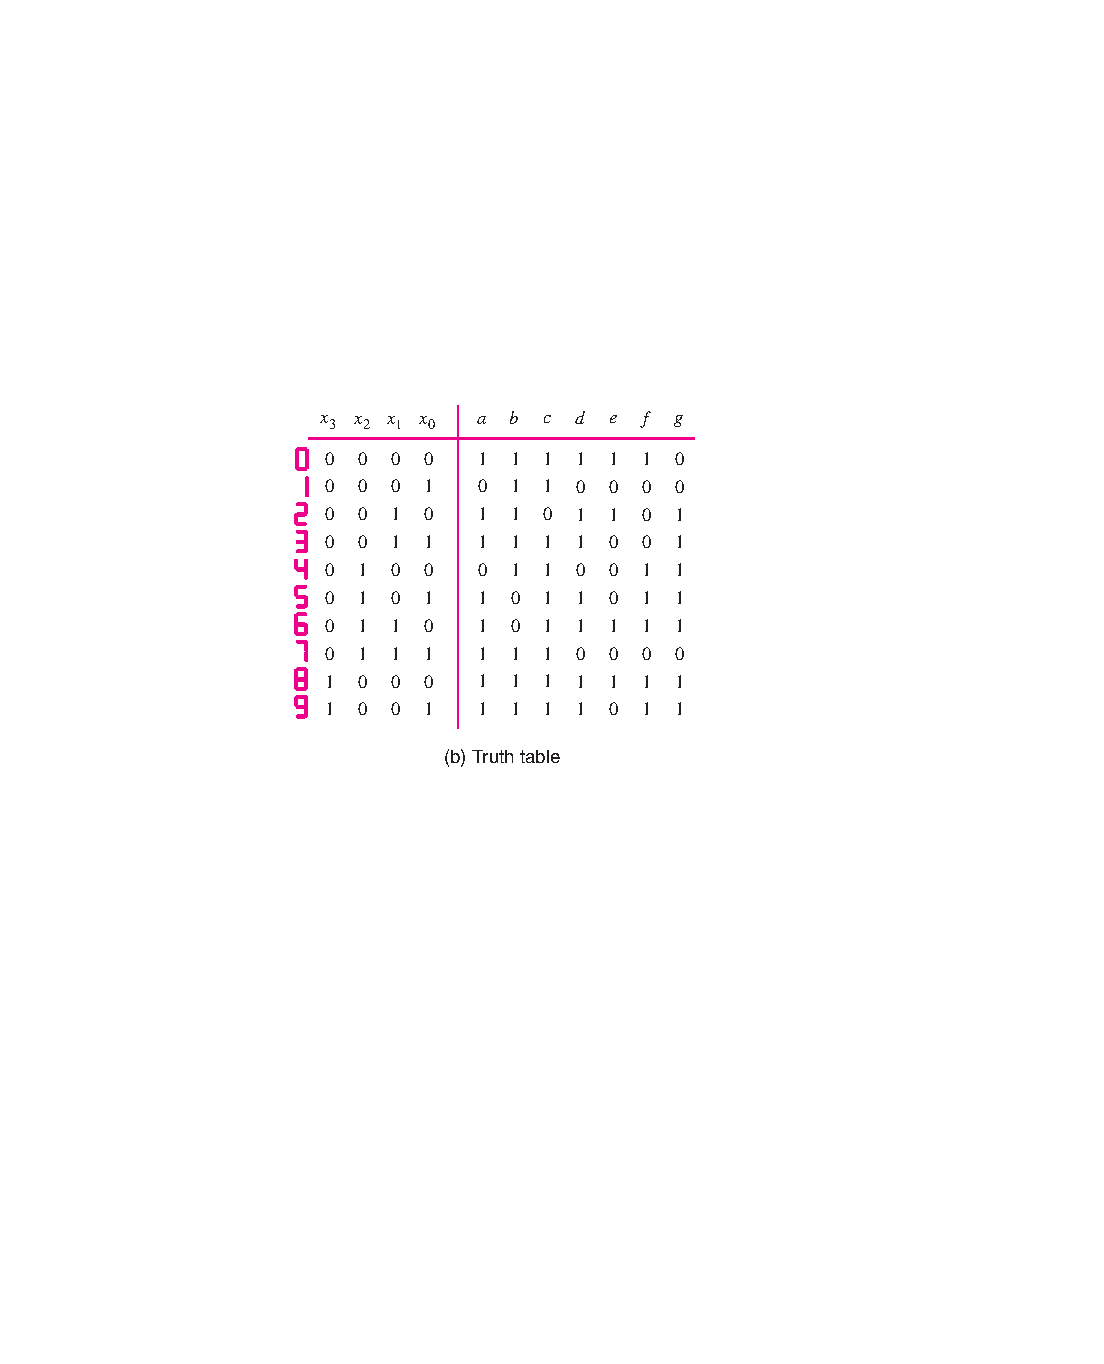
\includegraphics[width=.45\textwidth]{VerilogFig2_63b} 
\end{frame}

\begin{frame}{\insertsection} \centering
    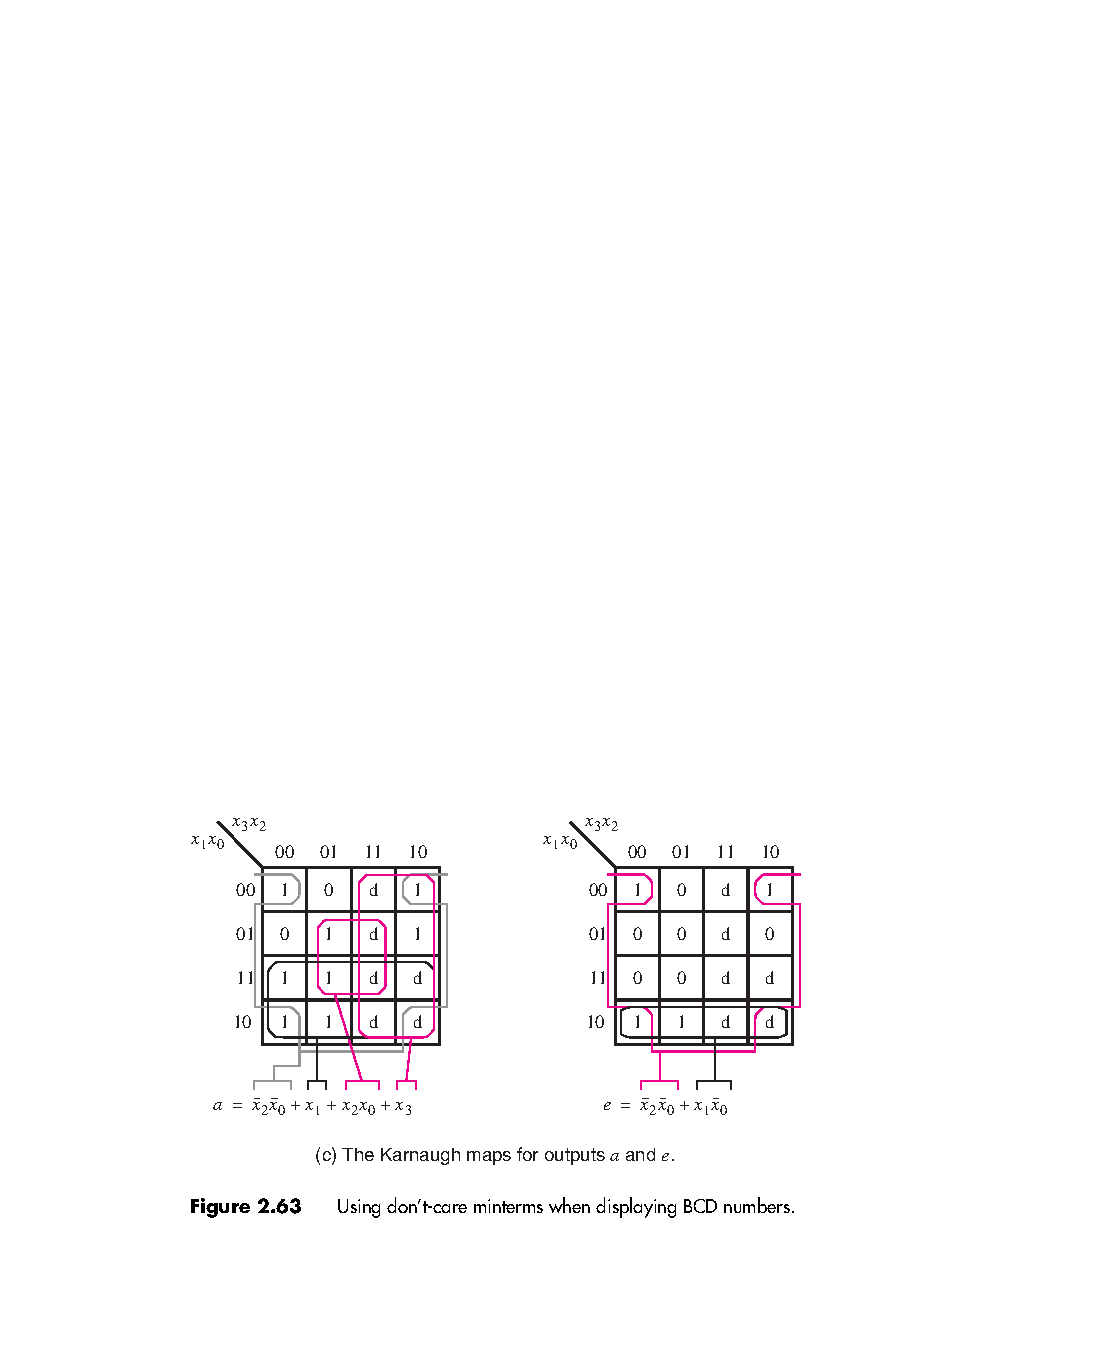
\includegraphics[width=.8\textwidth]{VerilogFig2_63c}
\end{frame}

\begin{frame}{\insertsection} 
    \begin{columns}
        \begin{column}{0.50\textwidth}
            \centering
            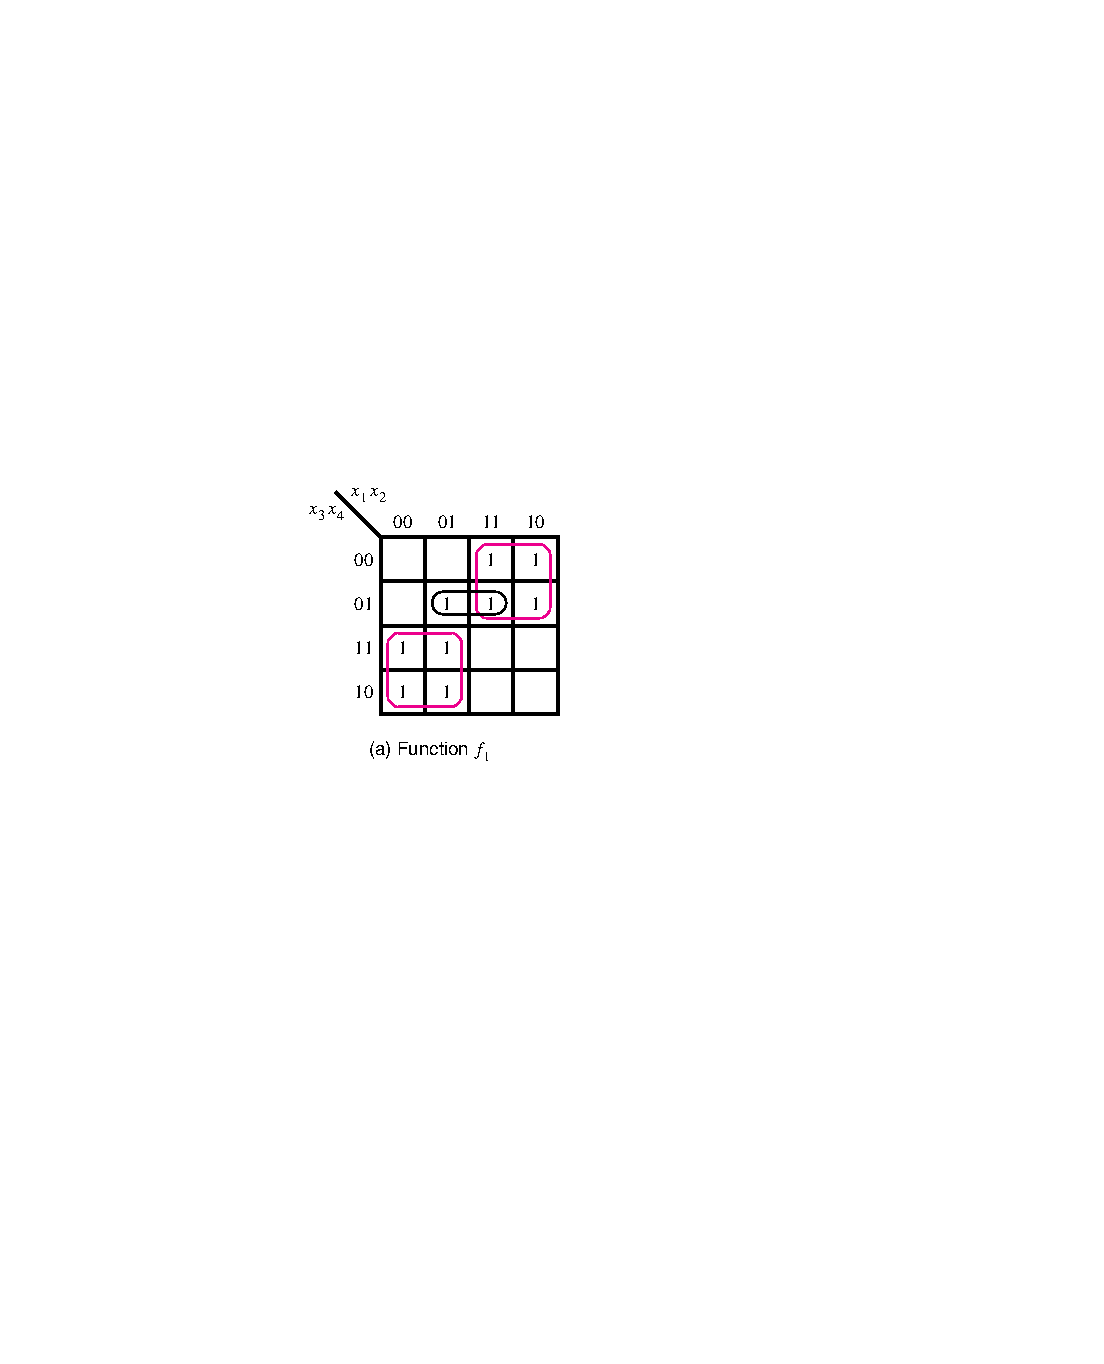
\includegraphics[width=.5\textwidth]{VerilogFig2_64a}
            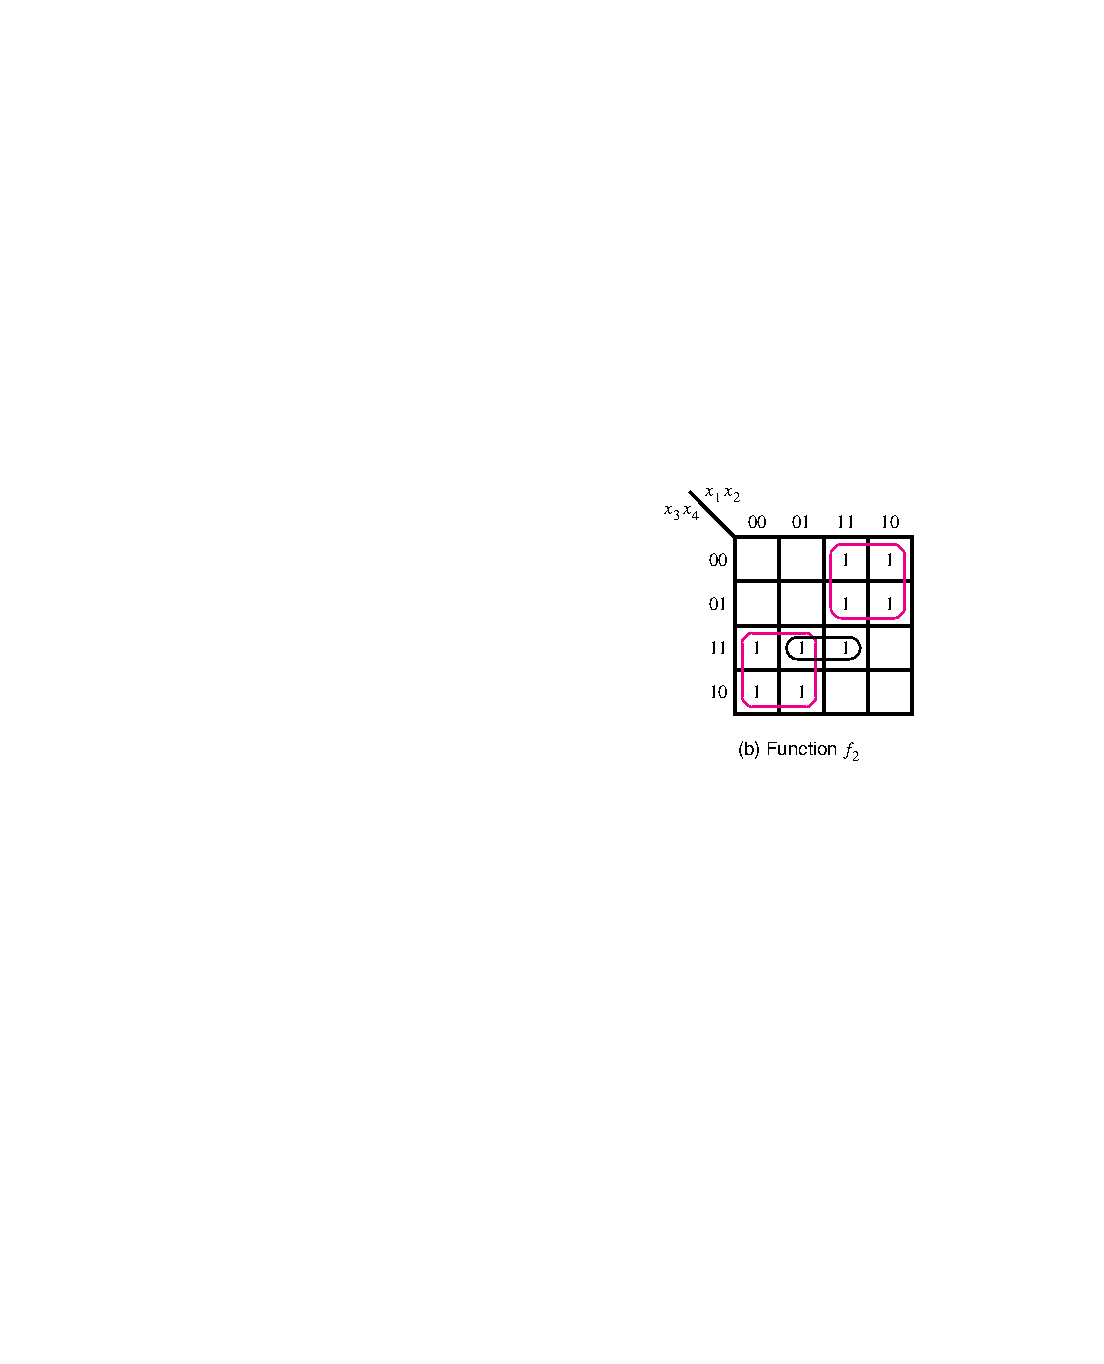
\includegraphics[width=.5\textwidth]{VerilogFig2_64b}
        \end{column}        
        \begin{column}{0.50\textwidth}
            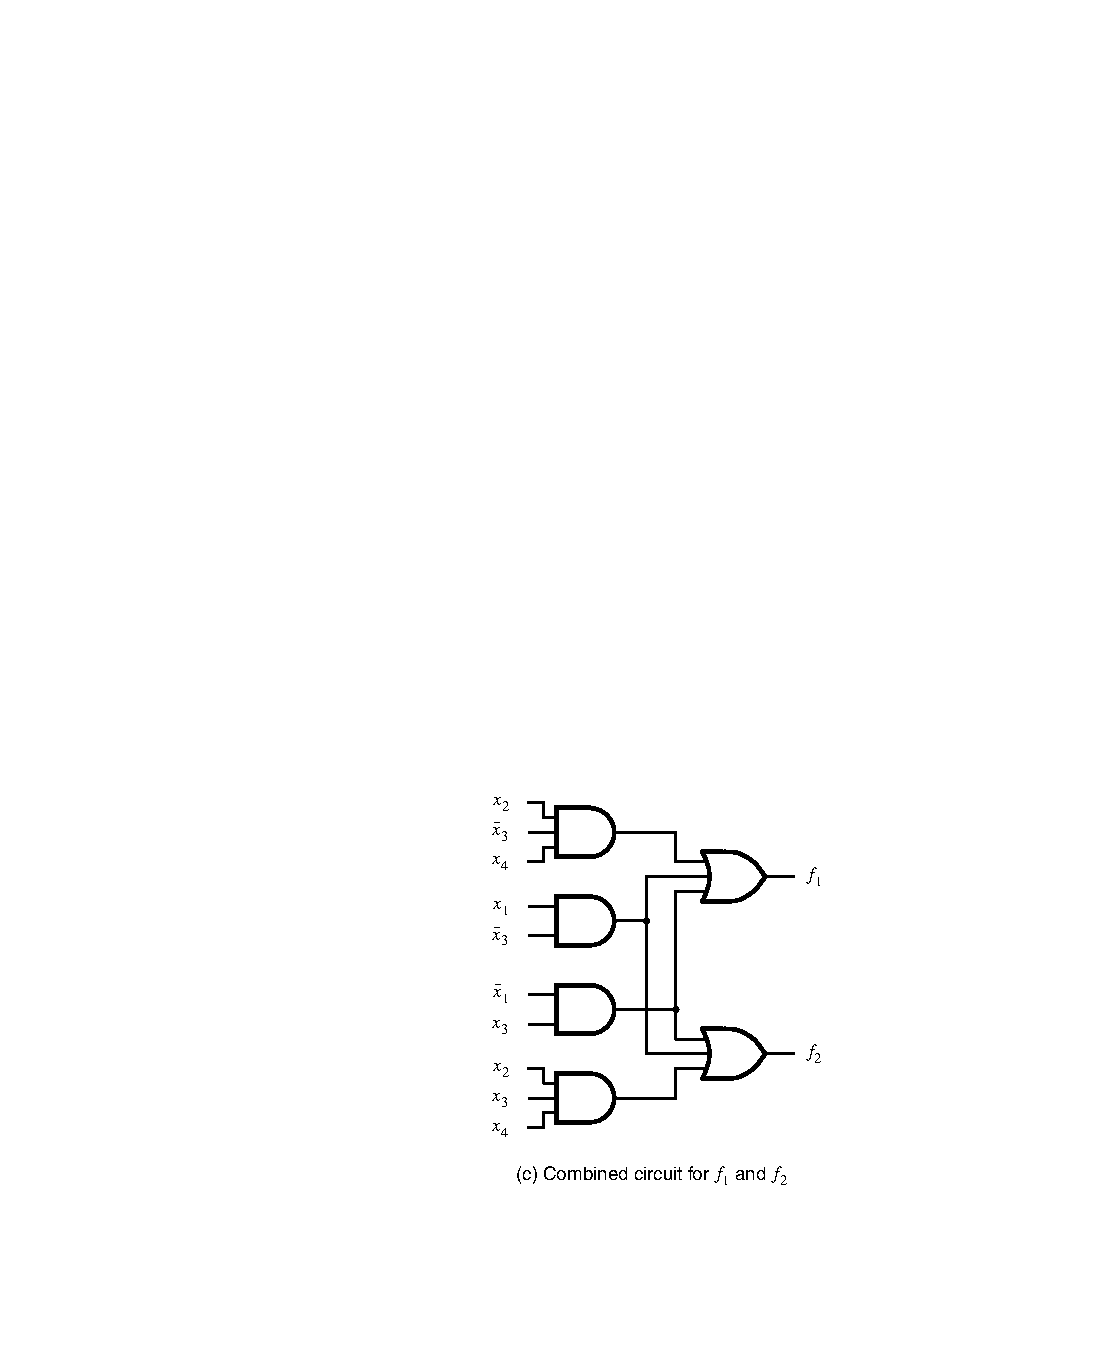
\includegraphics[width=.75\textwidth]{VerilogFig2_64c}
        \end{column}
    \end{columns}    
\end{frame}

\begin{frame}{\insertsection} \centering
    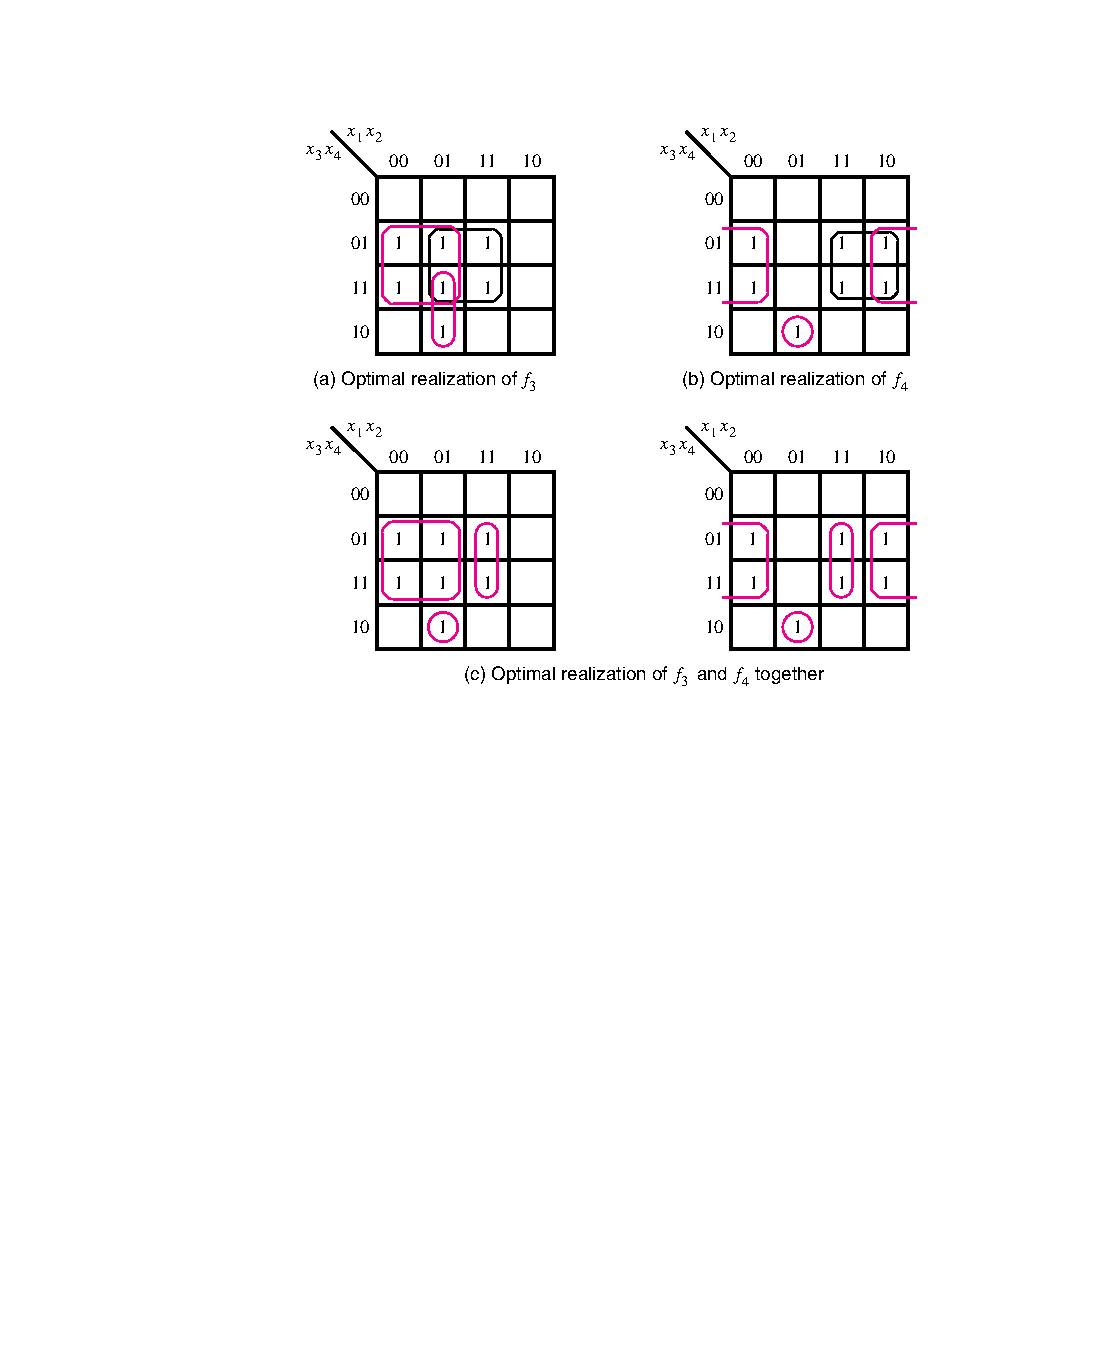
\includegraphics[width=.6\textwidth]{VerilogFig2_65abc}
    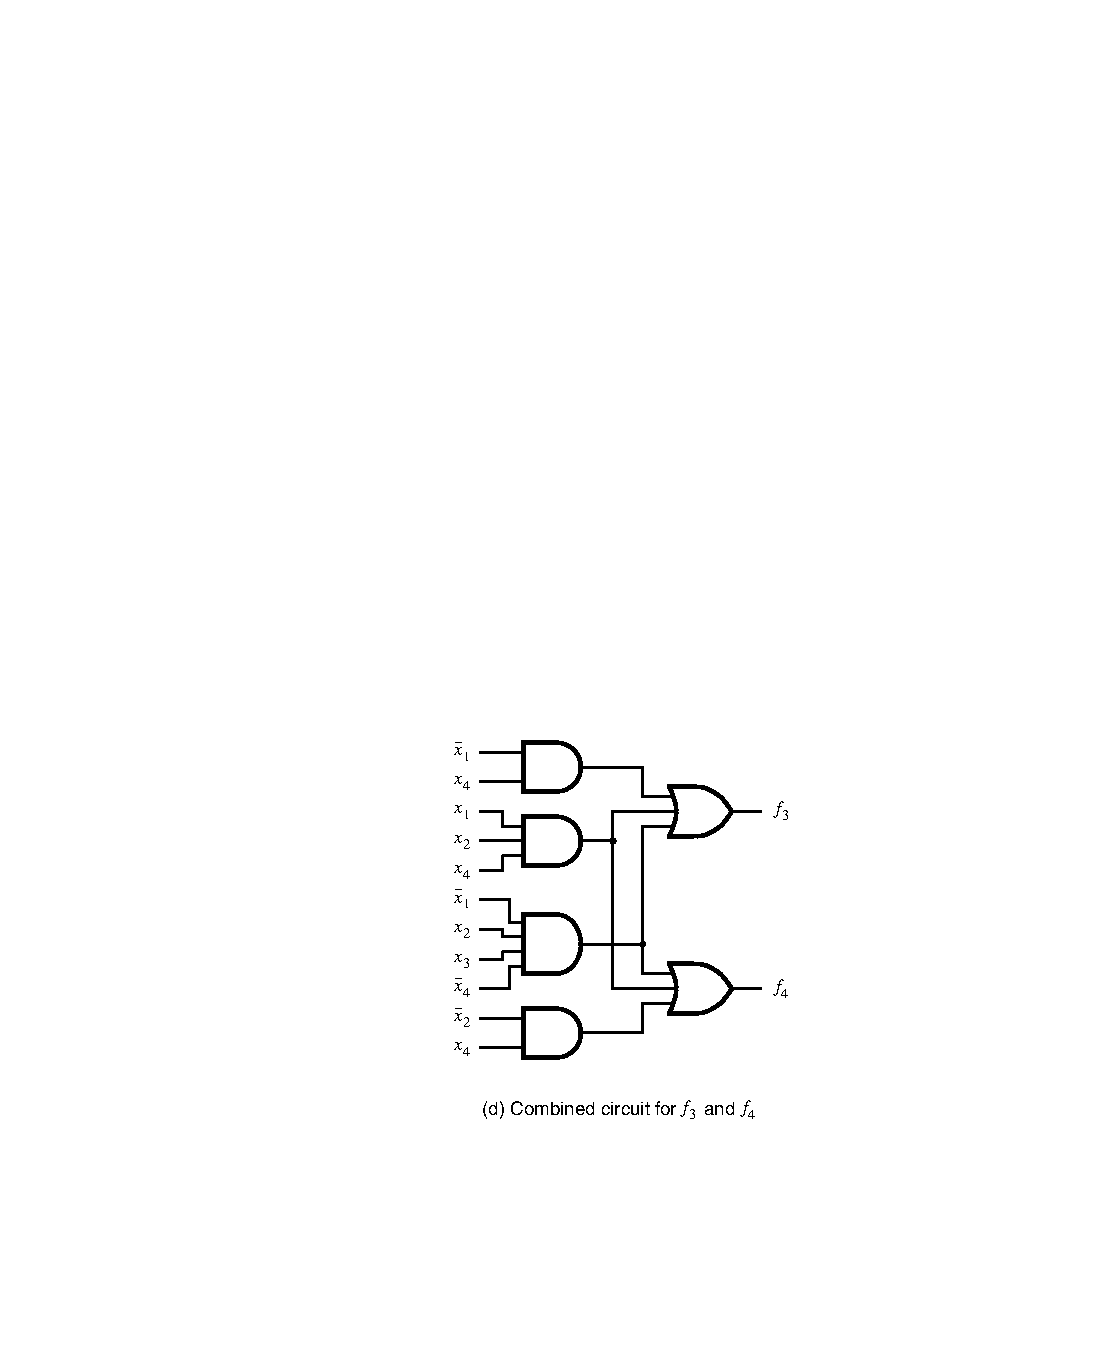
\includegraphics[width=.45\textwidth]{VerilogFig2_65d}
\end{frame}

% \begin{frame}{Frame Title}
%         \begin{tikzpicture}[circuit logic US, every circuit symbol/.style={thick}]
%         \node (a) at (0, 2) {$a$};
%         \node (b) at (0, 1) {$b$};
%         \node (c) at (0, 0) {$c$};
%         \node (f) at (4, 1) {$f$};
%         \pause
%         \node[not gate US, draw, thick] at ($(a) + (0.75, 0)$) (nota) {};
%         \node[and gate, inputs={nn}] at ($(b)!0.5!(c) + (1.5, 0)$) (and2) {};
%         \node[or gate, inputs={nn}] at ($(b) + (3, 0)$) (orb) {};
%         \pause
%         \draw[thick] (a) -- (nota.input);
%         \draw[thick] (nota.output) -- ($(nota.output) + (1, 0)$) |- (orb.input 1);
%         \draw[thick] (b) -- ($(b) + (0.75, 0)$) |- (and2.input 1);
%         \draw[thick] (c) -- ($(c) + (0.75, 0)$) |- (and2.input 2);
%         \pause
%         \draw[thick] (and2.output) -- ($(and2.output) + (0.25, 0)$) |- (orb.input 2);
%         \draw[thick] (orb.output) -- (f);
%     \end{tikzpicture} \\
    
% \end{frame}

%%%%%%%%%%%%%%%%%%%%%%%%%%%%%%%%%%%%%%%%%%%%%%%%%%%%%%%%%%%%%%%%%%%%%%%%%%%%%%%%

\section{Bibliografia} %%%%%%%

\begin{frame}{\insertsection} 
	\begin{itemize}
		\item \href{https://www.google.com.br/search?q=filetype\%3Apdf+Fundamentals+of+Digital+Logic+with+Verilog+Design+&oq=filetype\%3Apdf}{Brown, S. \& Vranesic, Z. - Fundamentals of Digital Logic with Verilog Design, 3rd Ed., Mc Graw Hill, 2009}
	\end{itemize}
\end{frame}

\begin{frame}
	\titlepage
\end{frame} 

\end{document}